
\documentclass[letterpaper,12pt]{article} 
\usepackage[utf8]{inputenc}
\usepackage[spanish]{babel}
\usepackage{amsmath}
\usepackage{amsfonts}
\usepackage{amssymb} 
\usepackage{algorithm2e}
\usepackage{algorithm}
\usepackage{algorithmic}
\usepackage{graphicx} 			%graficos
\usepackage[colorlinks=true, linkcolor=black, citecolor=black, urlcolor=blue]{hyperref} 	
\usepackage{wrapfig}
\usepackage{enumitem}
\usepackage{fancyhdr}
\usepackage{float}
\usepackage{eurosym}
\usepackage{color}
\usepackage{titling}
\usepackage{lipsum}
\usepackage{tocbibind}
\usepackage{longtable,multirow,booktabs}
\usepackage{multicol}

\usepackage[left=3cm,right=3cm,top=3cm,bottom=4cm]{geometry}		%margenes para documento


\pagestyle{fancy}													% estilo del estlo de pie cabezera


%%% Para las cabeceras
\newcommand{\hsp}{\hspace{20pt}}
\newcommand{\HRule}{\rule{\linewidth}{0.5mm}}
\headheight=50pt


\newcommand{\vacio}{\textcolor{white}{este es un texto que no se vera porque el colorde letra es blanco}} 			%comando para dar un texto 

\definecolor{rojoportada}{rgb}{0.9058 ,0.2980 , 0.23}				%color Rojo para las cabezeras


%====================================Datos del proyecto ======================================

%titulo del proyecto
\title{Sistema de Domotica  }				

%%%% AUTORES
\newcommand{\autorUno}{
	Univ. Alexander Mamani Y.\\
	FCyT\\
	Cocambamba\\
	akeymy4@gmail.com.}
\newcommand{\autorDos}{
	Univ. Ismael David.\\
	FCyT\\
	Cocambamba\\
	Isma@gmail.com.}
\newcommand{\autorTres}{
	Univ. Narriet Apellido .\\
	FCyT\\
	Cocambamba\\
	narriet@gmail.com.}




\begin{document}





{%\Large

\newpage

%%%Encabezamiento y pie de página
%%% También se genera automáticamente
%%% Mejor no tocarlo mucho.
\renewcommand{\headrulewidth}{0.5pt}
\fancyhead[L]{
	\textcolor{rojoportada}{\fontfamily{phv}\fontsize{14}{4}\selectfont{ \textbf{\thetitle}   }}\\
}
\fancyhead[R]{
	\textcolor{rojoportada}{\fontfamily{phv}\fontsize{14}{4}\selectfont{ \textbf{SCESI}   }}\\
}




%=================================pie de pagina==========================
\renewcommand{\footrulewidth}{0.5pt}
\fancyfoot[L]{
	\footnotesize SCESI\\
	Sociedad Cientifica de Estudiantes de Sistemas e Informatica\\
	http://www.scesi.org
}
\fancyfoot[C]{\vacio}														%hacemos uso del comando que creamo \vacio
\fancyfoot[R]{\footnotesize Página \thepage}								%numeracion de la pagina					
\
\vacio
\


\begin{center}
	\vspace{.5cm}
	{\fontfamily{phv}\fontsize{20}{5}\selectfont{\textsc{\thetitle}}}\\
	[2cm]		
	%importamos una imagen
	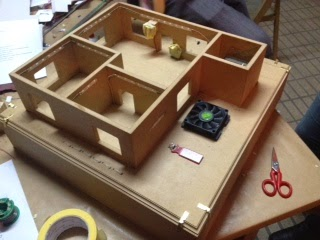
\includegraphics[width=5.5cm]{images/maqueta.jpeg}								
	\\[2cm]
	
	
	%\textcolor{azulportada}	

	
	Presentado por :
	\vspace{1.5cm}
	
	\begin{minipage}[b]{5.5cm}
		\begin{center}
			\autorUno
		\end{center}
	\end{minipage} \hfill \begin{minipage}[b]{4cm}
		\begin{center}
			\autorDos
		\end{center}
	\end{minipage} \hfill \begin{minipage}[b]{5cm}
		\begin{center}
			\autorTres
		\end{center}
		
	\end{minipage}\\
	[4cm]

	{\fontfamily{phv}\fontsize{12}{3}\selectfont{Cochabamba, 2018}}\\[1cm]
\end{center}



\vspace{1cm}
\ %% Así hago que se abra más espacio entre renglones.



\tableofcontents
\newpage



\section{INTRODUCCIÓN}
\vspace{1.5cm}

Las innovaciones tecnológicas siempre han sido aplicadas y utilizadas en las viviendas. Su incorporación ha contribuido a cambiar desde las relaciones familiares hasta la estructura de la ciudad.
 
Recientemente la domótica, o el uso y adopción de las nuevas tecnologías de la información y la comunicación en el hogar, está empezando a inducir cambios en el uso y la función de la vivienda, acentuando las alteraciones en la percepción del espacio-tiempo que ya se detectan en otras instancias de la vida cotidiana. 
 
 Se pude señalar entonces que la naturaleza y función de la vivienda está mutando considerablemente, lo cual plantea retos en la medida que constituye una de las instancias primarias de las relaciones sociales, de la interacción familiar, de la vida cotidiana y de la estructura de la ciudad



\section{ANTECENTES}
\section{JUSTIFICACION}
\section{PLANTEAMIENTO DEL PROBLEMA}
\section{OBJETIVOS}
\section{HIPOTESIS}
\section{NOVEDAD Y APORTE CIENTIFICO}
\section{METODOLÓGIA Y FUENTES}
\section{DESARROLLO DEL PROYECTO}
\section{CONCLUSIONES Y RECOMENDACIONES}






Las fuente de información que tomamos como base para desarrollar el proyecto son principalmente publicas y bibliográficas\\

Tambien para el desarrolo del proyecto se trabajo con la metodologia agil Scrum, puesto que era la que mas se adaptaba mas a nuestra comodidad.\\



Como Sistema de Control de Versiones se uso GitHub, ya que nos permite el trabajo colaborativo y no presencial(\url{https://github.com/akey96/TallerDeProgramacion}\\)


Para el desarrollo de la documentacion se uso el formato ACM.



%\section{CONCLUSIONES}

%\subsection{Resultados del desarrollo del proyecto}

%a que hemos llegado con esta investigacion y que podemos destacar de esta y problemas con los cuales nos topamos....
\newpage
\section{GLOSARIO DE TÉRMINOS}
\subsection{Diccionario}
\begin{itemize}
	
	\item \textbf{Arduino.- } Arduino es una plataforma de prototipos electrónica de código abierto (open – source) basada en hardware y software flexibles y  fáciles de usar. Está pensado e inspirado en artistas, diseñadores, y estudiantes de computación o robótica
	
	\item \textbf{Concurrecia.- } evento cuando  mas de un proceso intentan acceder al mismo recurso 
	
	\item \textbf{MVC .- }Arquitectura de software que separa los datos de una aplicación, la interfaz de usuario, y la lógica de control en tres componentes distintos.
	
	\item \textbf{Singleton.- } Es un patrón de diseño que permite restringir la creación de objetos pertenecientes a una clase o el valor de un tipo a un único objeto.Su intención consiste en garantizar que una clase solo tenga una instancia y proporcionar un punto de acceso global a ella.
	
	\item \textbf{Eficiencia Espacial.- }Cantidad de recursos espaciales ( de  almacén) que un algoritmo consume o necesita para su 
	ejecución
	
	\item \textbf{SCV.- }  Software que administra el acceso a un conjunto de ficheros, y mantiene un historial de cambios realizados. El control de versiones es útil para guardar cualquier documento que cambie con frecuencia, como código fuente, documentación o ficheros de configuración.
	
	\item \textbf{XML.- } XML proviene de eXtensible Markup Language (“Lenguaje de Marcas Extensible”). Se trata de un metalenguaje (un lenguaje que se utiliza para decir algo acerca de otro) extensible de etiquetas que fue desarrollado por el Word Wide Web Consortium (W3C)
	
	\item \textbf{Comunicacion Asincrona.- }Es la conexión que se establece entre el cliente y el servidor que permite la transferencia de datos no sincrónica, o sea el cliente puede realizar varias peticiones al servidor sin necesidad de esperar por la respuesta de la primera. 
	
		
\end{itemize}

\newpage


\section{BLIBLIOGRAFIA}

%\renewcommand\refname{Bibliografía}

\begin{thebibliography}{9}
%\bibitem(Vesperman,2007){Vesperman} J. Vesperman. “Essential CVS”. O’Really Media Inc, 2007.
\bibitem{Singleton}{mundoerp} http://mundoerp.com/blog/Singleton
\bibitem{Arduino}{arduinodhtics} https://arduinodhtics.weebly.com/iquestqueacute-es.html
\bibitem{xml}{definicion} https://definicion.de/xml/
\bibitem{Comunicacion Asincrona}{ecured} https://www.ecured.cu/Comunicaci\%C3\%B3n\_as\%C3\%ADncrona
\bibitem{SCV}{mundoerp} http://mundoerp.com/blog/sistemas-de-control-de-versiones/
\end{thebibliography}

\newpage

\end{document}

